% -*- TeX-master: "main"; fill-column: 72 -*-

\section{Examples}
\label{examples}


This proposal mainly covers logical models but it can also handle standard Petri nets. We provide one toy example of each and the logical model of the decision between lysis and lysogenization in temperate bacteriophage as defined by \citet{thieffry95}.
%the examples are labeled with a token indicating the corresponding formalism : \ALL all formalisms, \PN Petri nets, \LRG logical regulatory networks or \SYM symbolic relationships.

\subsection{Simple Logical Regulatory Graph} % (fold)
\label{sub:lrg}
%\LRG 
The following example shows a simple LRG with 3 regulators A, B and C, where A can take three values ($A=\{0,1,2\}$), and B,C are Boolean. Moreover, A positively regulates B, which positively regulates C, which positively regulates A. In turn A activates itself at level 1 but inhibits itself at a higher level (2) as illustrated by \ref{ex-lrg}.

\begin{figure}[hb]
  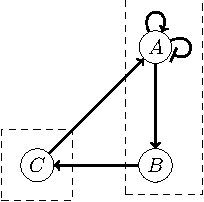
\includegraphics{figs/LRG.pdf}
  \caption{A simple Logical Regulatory Network.}
  \label{ex-lrg}
\end{figure}


The logical functions are the following:

\smallskip

\begin{center}


%$
%A_{t+1} :=\left\{ \begin{array}{cl}
%      2 & \mbox{if $(1 <= A_t < 2)$ or $((C_t >= 1)$ and $(A_t >= 1))$} \\
%      1 & \mbox{if $(A_t < 1)$ and $(C_t >= 1)$} \\
%      0 & \mbox{otherwise}  \\
%     \end{array}
%\right.
%$
%\end{center}
%\begin{center}
%$
%B_{t+1} :=\left\{ \begin{array}{cl}
%      1 & \mbox{if $A_t >= 1$} \\
%      0 & \mbox{otherwise}  \\
%     \end{array}
%\right.
%$
%\end{center}
%\begin{center}
%$
%C_{t+1} :=\left\{ \begin{array}{cl}
%      1 & \mbox{if $B_t >= 1$} \\
%      0 & \mbox{otherwise}  \\
%     \end{array}
%\right.
%$


$
\begin{array}{l}

A_{i+1} :=\left\{ \begin{array}{cl}
      2 & \mbox{if $(1 <= A_i < 2)$ or $((C_i >= 1)$ and $(A_i >= 1))$} \\
      1 & \mbox{if $(A_i < 1)$ and $(C_i >= 1)$} \\
      0 & \mbox{otherwise}  \\
     \end{array}
\right.
B_{i+1} :=\left\{ \begin{array}{cl}
      1 & \mbox{if $A_i >= 1$} \\
      0 & \mbox{otherwise}  \\
     \end{array}
\right.
C_{i+1} :=\left\{ \begin{array}{cl}
      1 & \mbox{if $B_i >= 1$} \\
      0 & \mbox{otherwise}  \\
     \end{array}
\right.
\end{array}
$

\end{center}

\bigskip

The state transition tables are thus:

\bigskip

\begin{center}\begin{tabular}{ccc}
\begin{tabular}{|c|c||c|}
$A_i$&$C_i$&$A_{i+1}$   \\\hline
0&0&0 \\
0&1& 1\\
1&0&2 \\
1&1&2 \\
2&0& 0\\
2&1&2 \\\hline
\end{tabular}
&
\begin{tabular}{|c||c|}
$A_i$&$B_{i+1}$  \\\hline
0&0 \\
1& 1\\
2& 1\\\hline
\end{tabular}
&
\begin{tabular}{|c||c|}
$B_i$&$C_{i+1}$  \\\hline
0& 0\\
1& 1\\\hline
\end{tabular}
\end{tabular}
\end{center}

\bigskip


\lstinputlisting[caption=Logical Regulatory Graph example,label=ex_LRG]{Examples/example.sbml}

% subsection lrg (end)
\bigskip
\subsection{Simple Petri net} % (fold)
\label{sub:ex_pn}
%\PN 
The following example shows a simple, standard Petri net, with 4 places A, B, C and D and one transition $t1$ as depicted in \ref{ex-pn}.
\begin{figure}[hb]
  
\includegraphics{figs/PN.pdf}
  \caption{A Petri net model.}
  \label{ex-pn}
\end{figure}

\bigskip
\lstinputlisting[caption=Petri net example,label=ex_pn_listing]{Examples/examplePetri.sbml}

% subsection ex_pn (end)


\bigskip
\subsection{Logical model of the immunity control in bacteriophage lambda}
\label{sub:ex_phage}
This last example is the multi-valued, logical model as defined by \citet{thieffry95} for the core network controlling the decision between lysis and lysogeny in temperate bacteriophage. 

\begin{figure}[hb]
  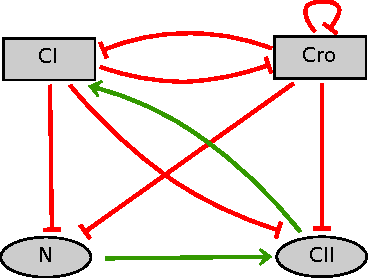
\includegraphics{figs/phage_lambda.pdf}
  \caption{Interaction graph of the four-variable multi-valued model of phage lambda switch \citep{thieffry95}.}
  \label{ex-phage}
\end{figure}

\lstinputlisting[caption= Phage lambda switch example,label=ex_phage_listing]{Examples/phage_lambda.sbml}



% subsection ex_phage (end)

% section use-cases and examples (end)
